\documentclass{article}
\usepackage{amsmath}
\usepackage{graphicx}
\usepackage{epstopdf}
\usepackage{float}
\usepackage{subcaption}
\usepackage{tikz}
\usepackage{ifthen}
\usepackage{color}
\usepackage{graphicx}
\newcommand{\myScale}{0.56}
\title{CSL603 - Lab 3\\Multi Layer Perceptron}
\author{Aditya Gupta\\2015CSB1003}
\begin{document}
\maketitle
\section{2-Dimensional 3-Class Classification problem}
\subsection{Goal} Study the changes to the 
\begin{itemize}
\item decision boundary and 
\item the training error
\end{itemize} with respect to parameters such as 
\begin{itemize}
\item number of training iterations,
\item number of hidden layer neurons and
\item finally the learning rate
\end{itemize}
\subsection{MLP Training}
During forward pass, we made $z_h=\sigma(w_h^Tx)$, $y'_k=\exp(v_k^Tz)/\sum_{k'=1}^K \exp(v_{k'}^Tz)$ (The weights and points had different orientation to what discussed in class, therefore an appropriate formula equivalent to these was used.)
During backpropagation, for a particular point we used $$\Delta v_{hk}=\underbrace{\eta(y'_k-y_k)}_{\text{Common for a particular } k}z_h$$, $$\Delta w_{jh}=\underbrace{\eta\left(\sum_k(y'_k-y_k)v_{hk}\right)z_h(1-z_h)}_{\text{Common for a particular }h}x_j$$ (Various values were calculated only once which were common for a particular $k$ for $\Delta v_{hk}$ and these were further used in case of $\Delta w_{jh}$, moreover the common values in case of $\Delta w_{jh}$ for a particular $h$ were also calculated only once.)
\subsection{Training Error}
The training error was calculated as $E(w,v)=-\sum_{k=1}^K y_k\log y'_k$ for a particular point that was trained in this epoch.
\subsection{MLP Testing}
The similar formulas as for MLP training were used but here, instead we had multiple points, so an appropriate form was used (The bias term was introduced differently which in this case would be a column vector, rest was same).
\subsection{Observations}
\subsubsection{Varying the number of hidden layer nodes}
The following figures depict the change in the sum of squared error vs. the number of training iterations for a particular $\eta$ value and varying the number of hidden layer nodes in powers of $2$:
\begin{figure}[H]
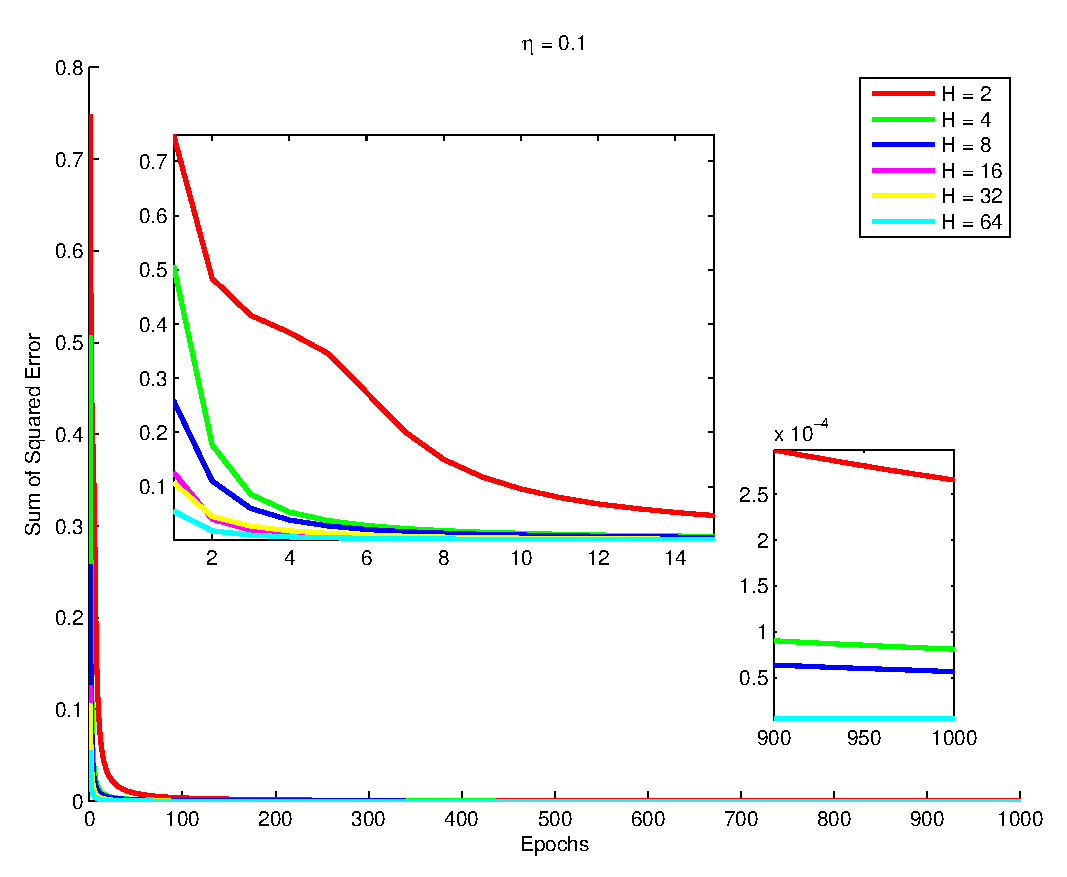
\includegraphics[scale=\myScale]{{../eps2/eta0.100000}.eps}
\caption{Change in Sum of Squared Error vs the Training Iterations for different values of H. $\eta=0.1$}
\label{fig:fig1}
\end{figure}
\begin{figure}[H]
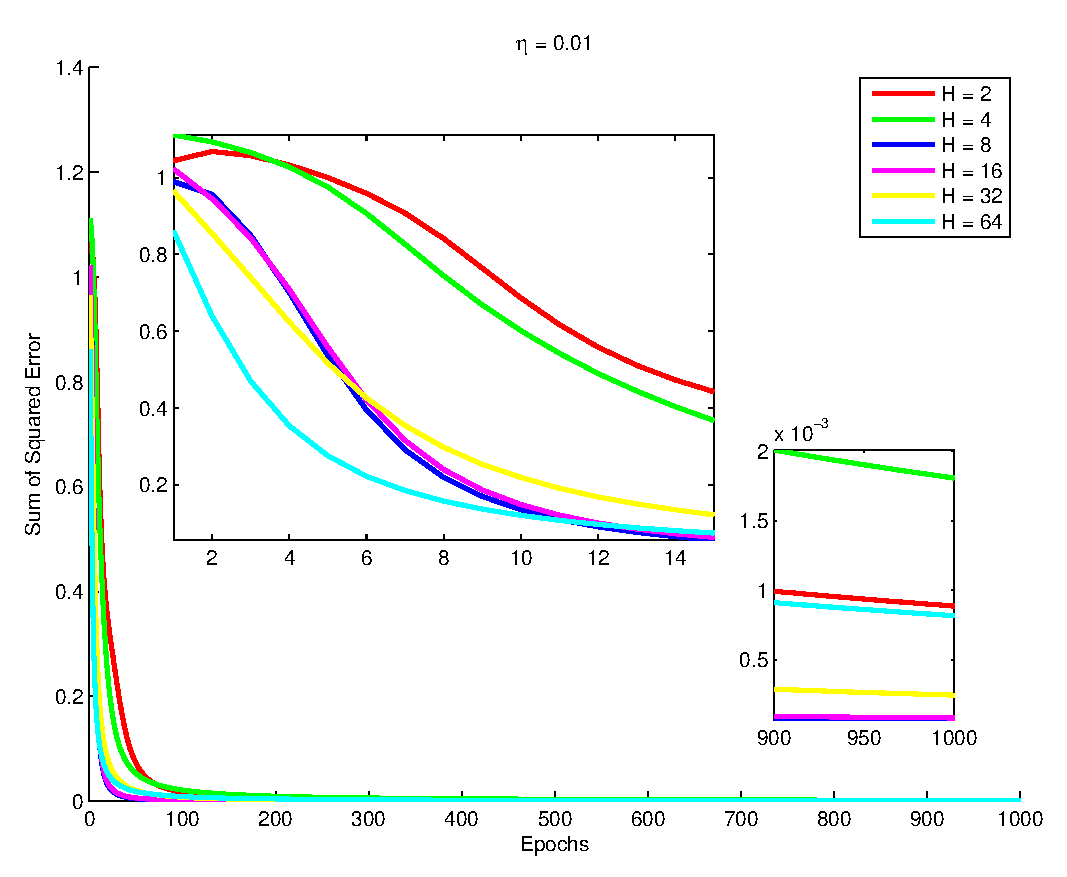
\includegraphics[scale=\myScale]{{../eps2/eta0.010000}.eps}
\caption{Change in Sum of Squared Error vs the Training Iterations for different values of H. $\eta=0.01$}
\label{fig:fig2}
\end{figure}
\begin{figure}[H]
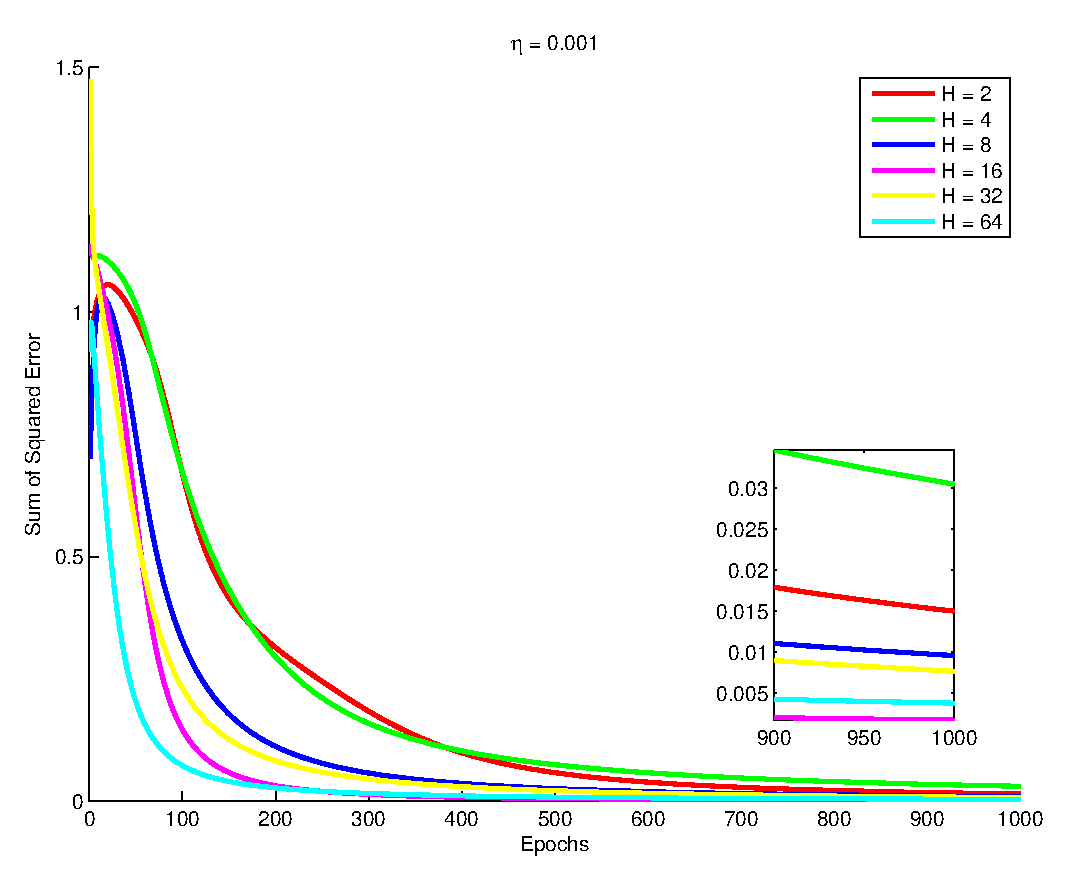
\includegraphics[scale=\myScale]{{../eps2/eta0.001000}.eps}
\caption{Change in Sum of Squared Error vs the Training Iterations for different values of H. $\eta=0.001$}
\label{fig:fig3}
\end{figure}
\begin{figure}[H]
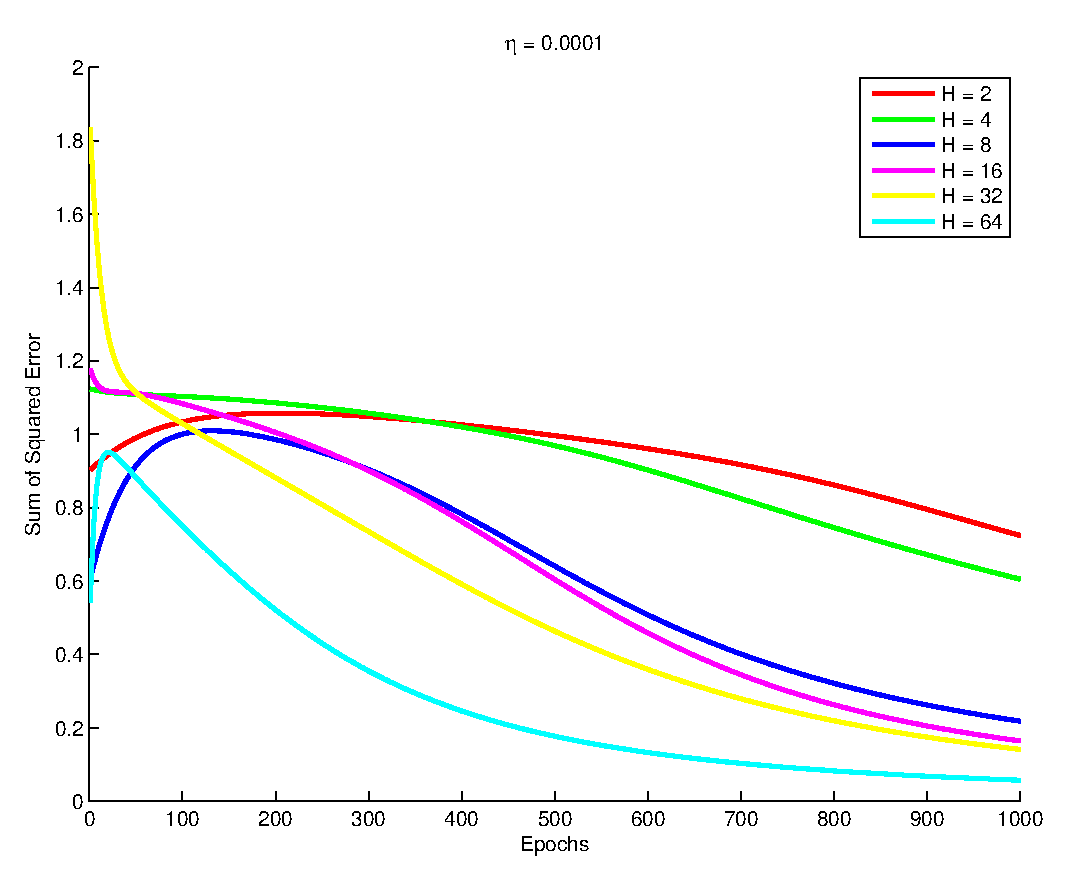
\includegraphics[scale=\myScale]{{../eps2/eta0.000100}.eps}
\caption{Change in Sum of Squared Error vs the Training Iterations for different values of H. $\eta=0.0001$}
\label{fig:fig4}
\end{figure}
\begin{figure}[H]
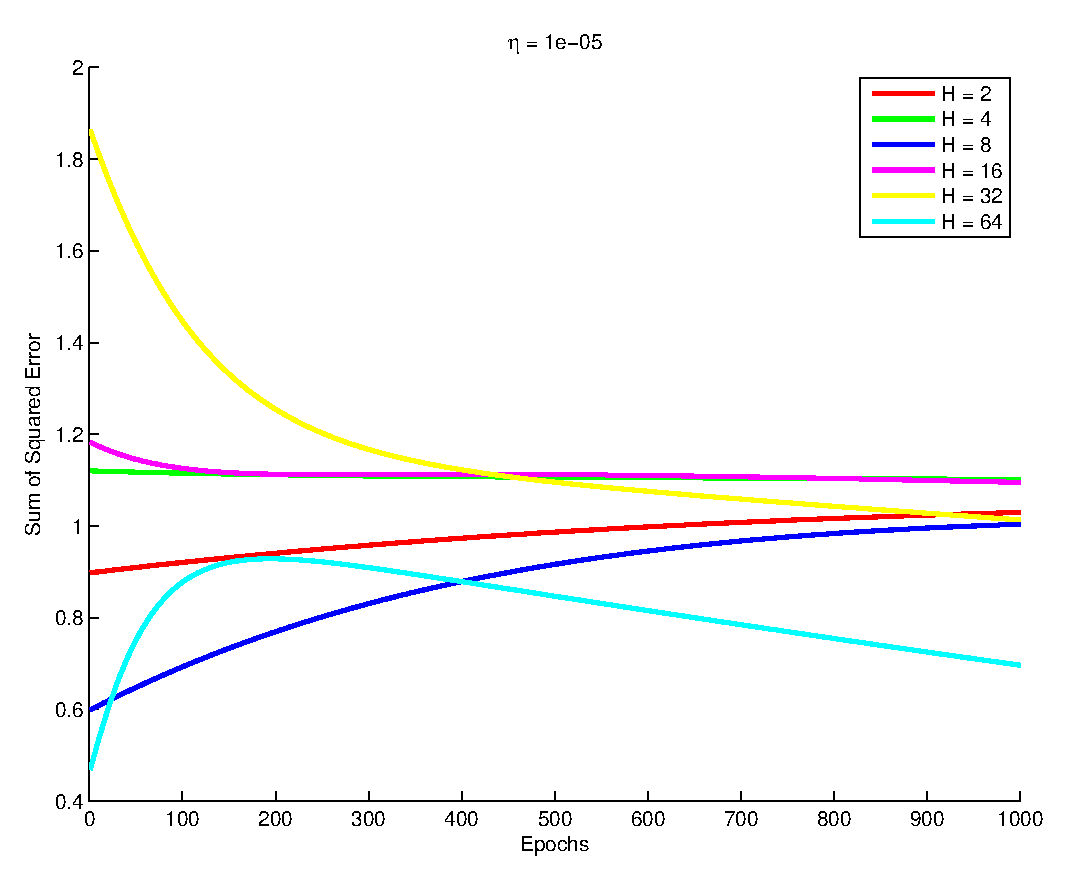
\includegraphics[scale=\myScale]{{../eps2/eta0.000010}.eps}
\caption{Change in Sum of Squared Error vs the Training Iterations for different values of H. $\eta=0.00001$}
\label{fig:fig5}
\end{figure}

\subsubsection{Varying the learning rate}
The following figures depict the change in the sum of squared error vs. the number of training iterations for a particular value of $H$ and varying the $\eta$:
\begin{figure}[H]
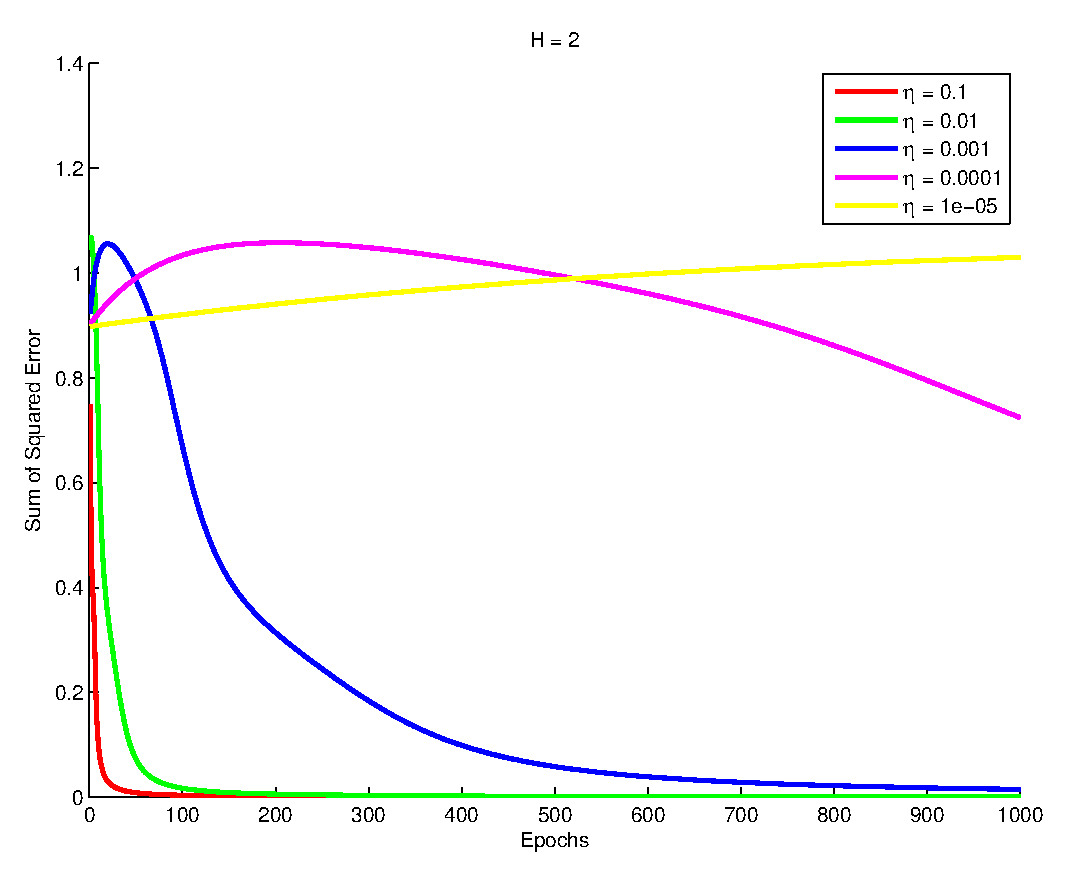
\includegraphics[scale=\myScale]{../eps2/H2.eps}
\caption{Change in Sum of Squared Error vs the Training Iterations for different values 
of $\eta$. $H=2$}
\label{fig:fig6}
\end{figure}
\begin{figure}[H]
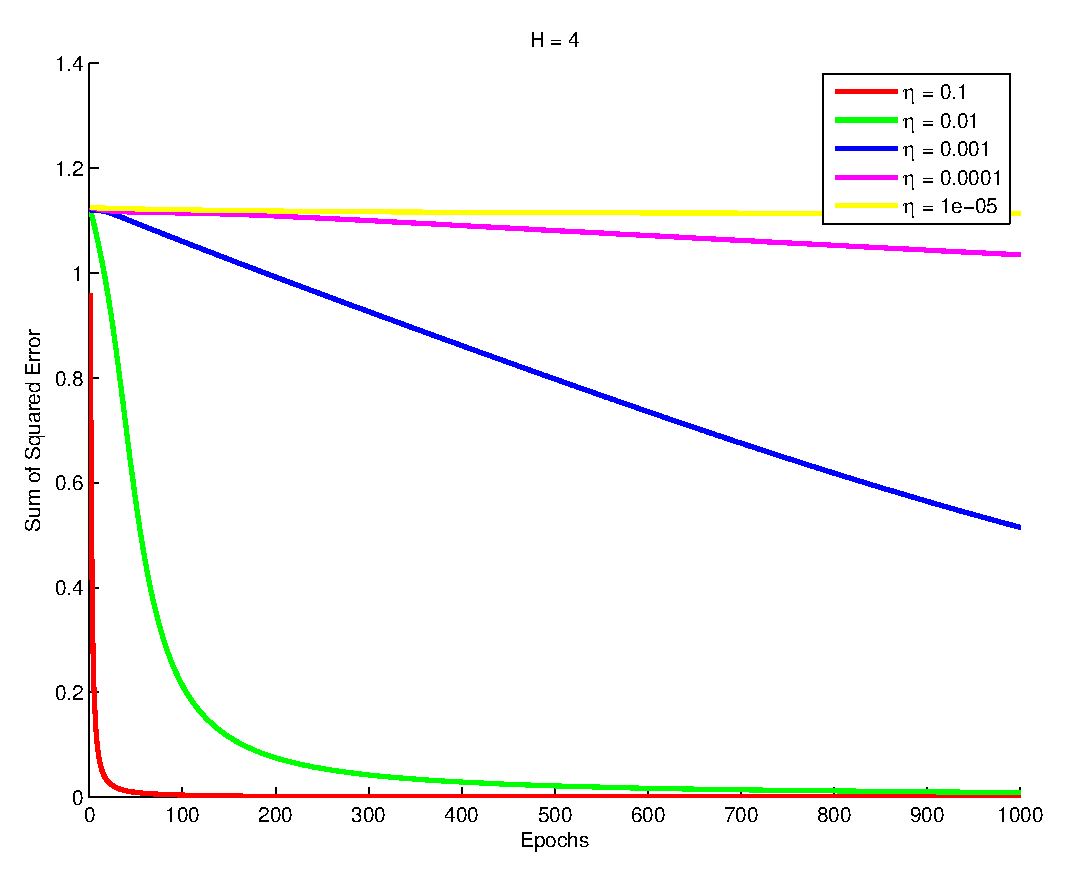
\includegraphics[scale=\myScale]{../eps2/H4.eps}
\caption{Change in Sum of Squared Error vs the Training Iterations for different values of $\eta$. $H=4$}
\label{fig:fig7}
\end{figure}
\begin{figure}[H]
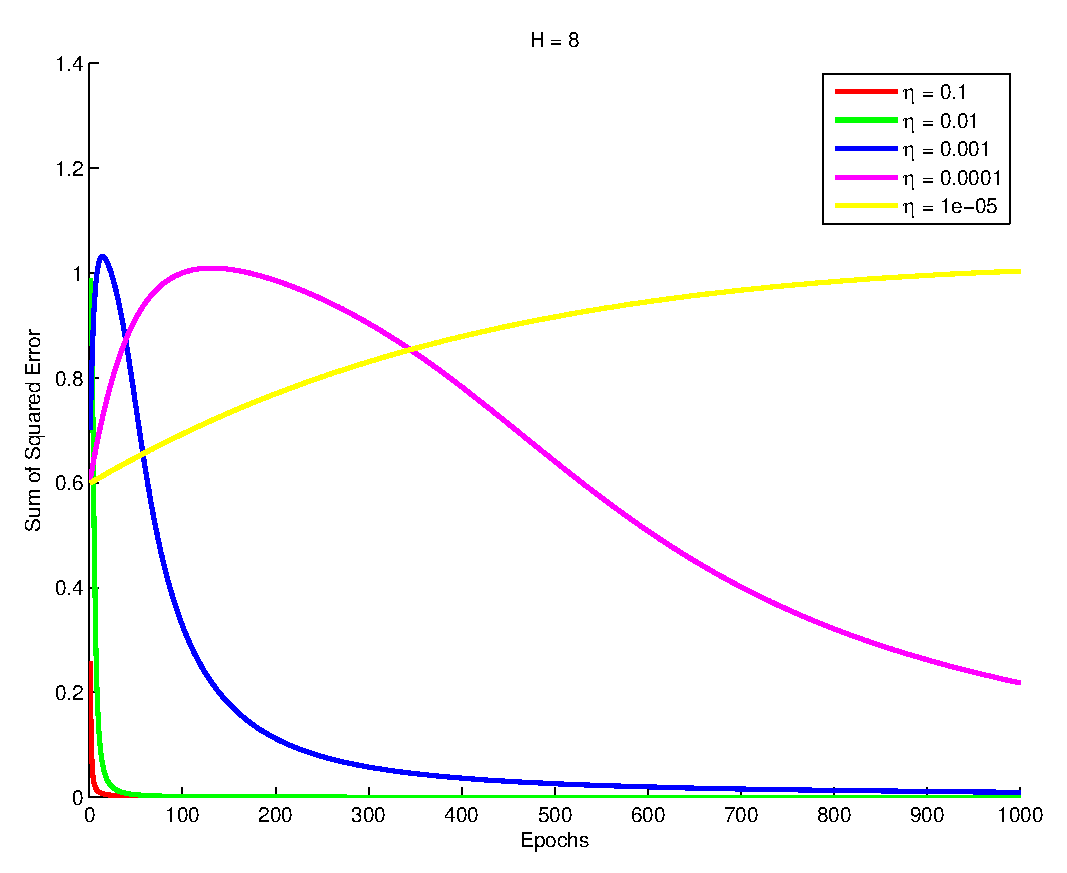
\includegraphics[scale=\myScale]{../eps2/H8.eps}
\caption{Change in Sum of Squared Error vs the Training Iterations for different values of $\eta$. $H=8$}
\label{fig:fig8}
\end{figure}
\begin{figure}[H]
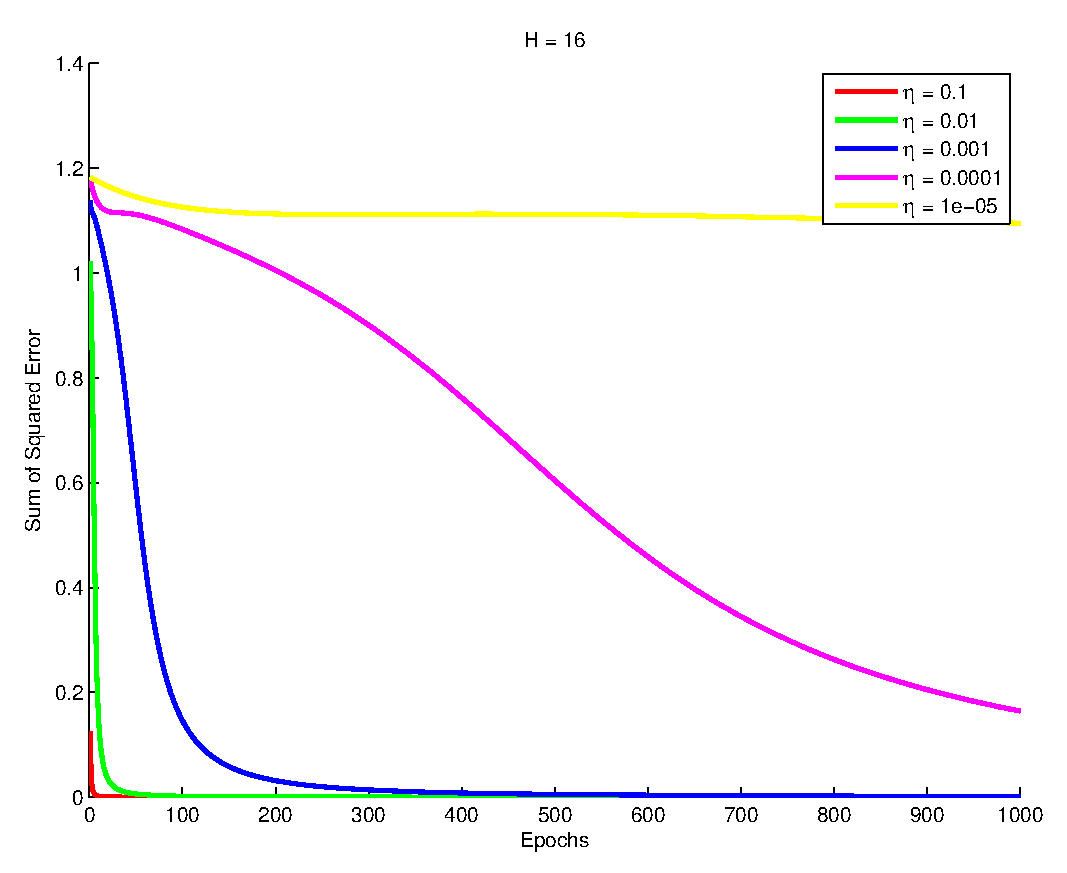
\includegraphics[scale=\myScale]{../eps2/H16.eps}
\caption{Change in Sum of Squared Error vs the Training Iterations for different values of $\eta$. $H=16$}
\label{fig:fig9}
\end{figure}
\begin{figure}[H]
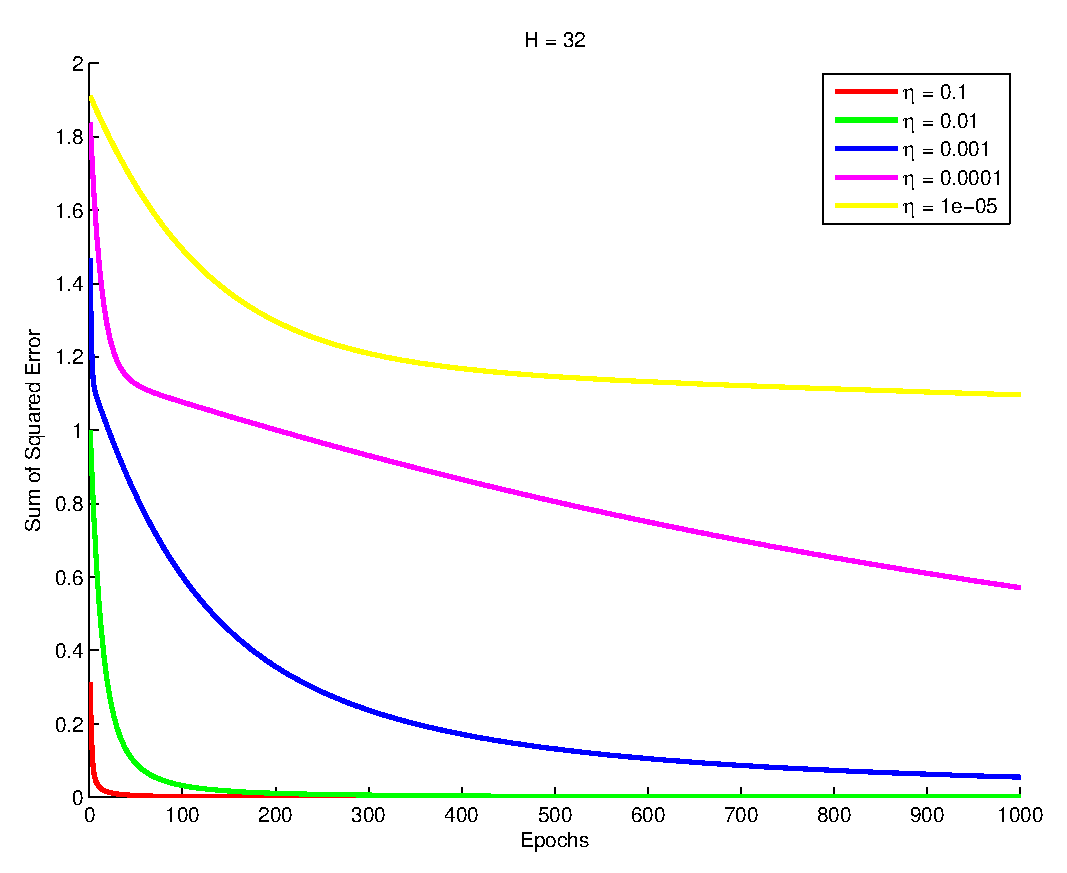
\includegraphics[scale=\myScale]{../eps2/H32.eps}
\caption{Change in Sum of Squared Error vs the Training Iterations for different values of $\eta$. $H=32$}
\label{fig:fig10}
\end{figure}
\begin{figure}[H]
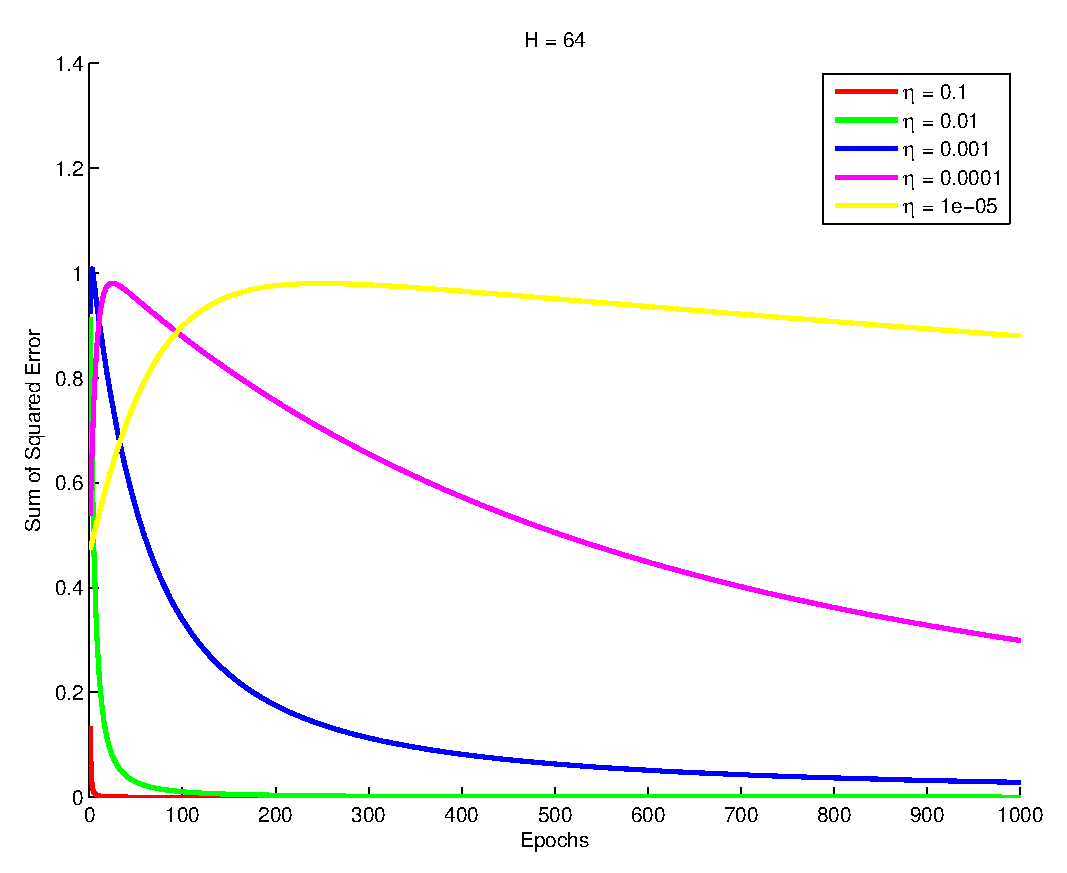
\includegraphics[scale=\myScale]{../eps2/H64.eps}
\caption{Change in Sum of Squared Error vs the Training Iterations for different values of $\eta$. $H=64$}
\label{fig:fig11}
\end{figure}

\subsubsection{Varying the training iterations}
The observations for the change in the sum of squared error by varying the training iterations can be made through the previous graphs.

\subsubsection{Change in Decision Boundary}
The change in decision boundaries for various values of $H$  and $\eta$ can be seen in the following graphs. Here red dots represent Class 1, green pluses represent Class 2 and blue circles represent Class 3.

\begin{figure}[H]
\minipage{0.32\textwidth}
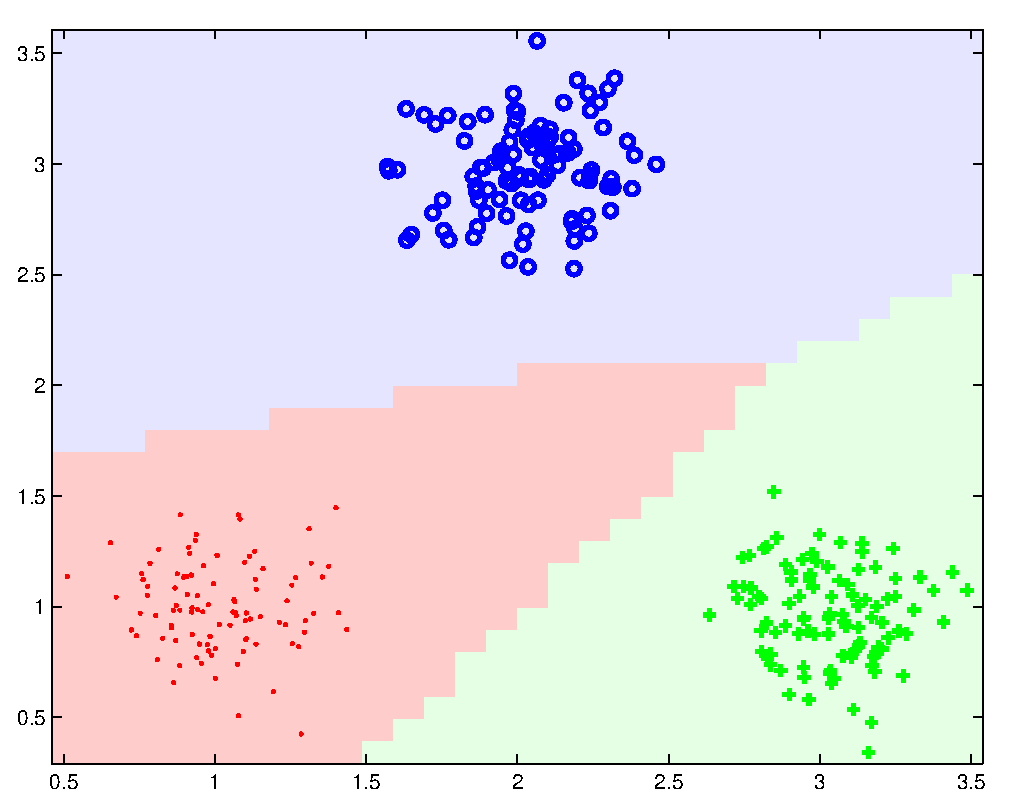
\includegraphics[scale=0.25]{{../eps/fig2_H2_eta0.010000}.eps}
\subcaption{ $H=2$}
\endminipage\hfill
\minipage{0.32\textwidth}
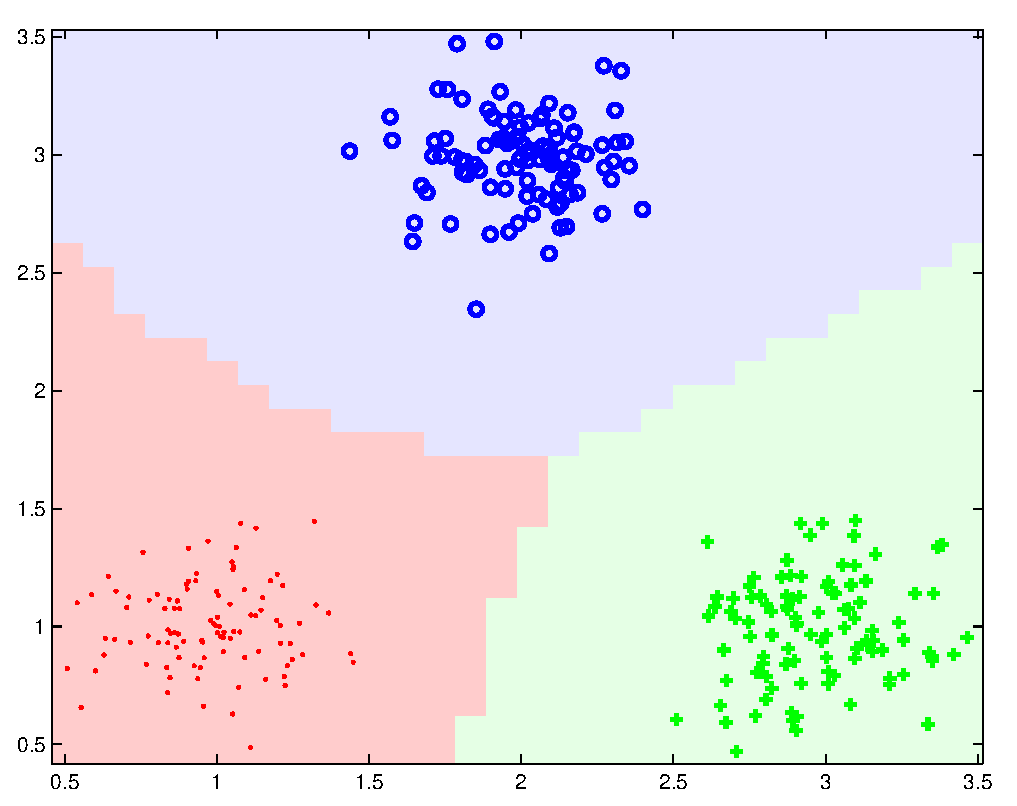
\includegraphics[scale=0.25]{{../eps/fig2_H4_eta0.010000}.eps}
\subcaption{ $H=4$}
\endminipage\hfill
\minipage{0.32\textwidth}
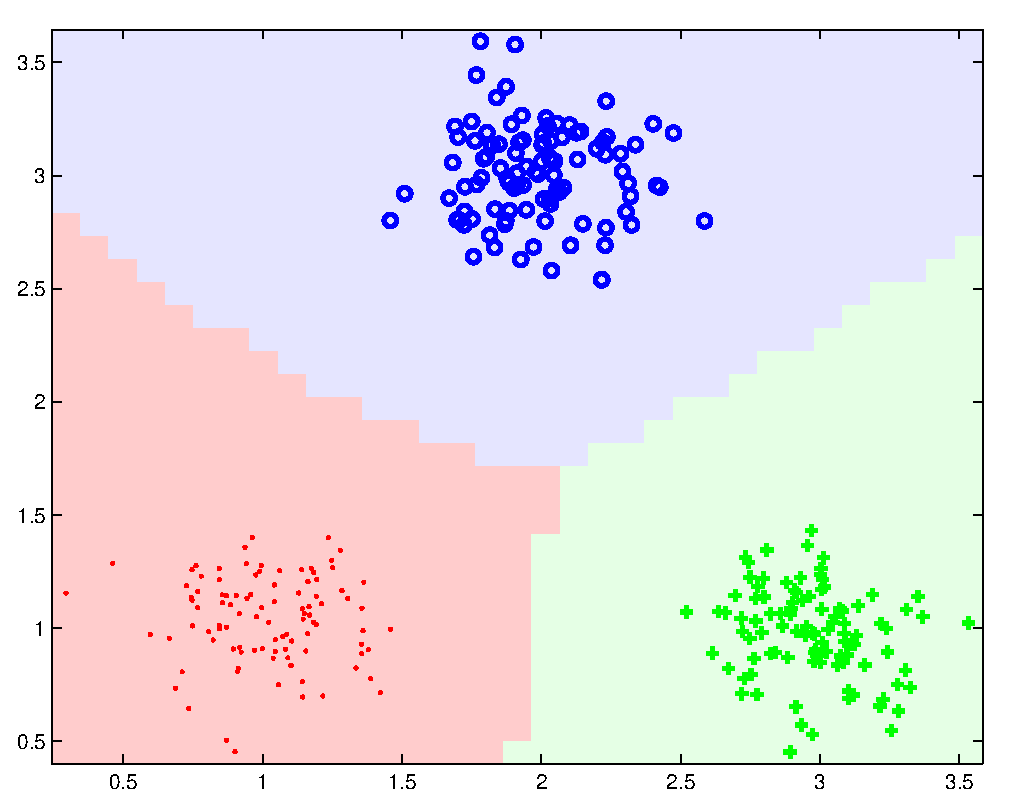
\includegraphics[scale=0.25]{{../eps/fig2_H64_eta0.010000}.eps}
\subcaption{ $H=64$}
\endminipage\hfill
\caption{Deicision boundary for $\eta=0.01$}
\label{fig:fig12}
\end{figure}

\begin{figure}[H]
\minipage{0.32\textwidth}
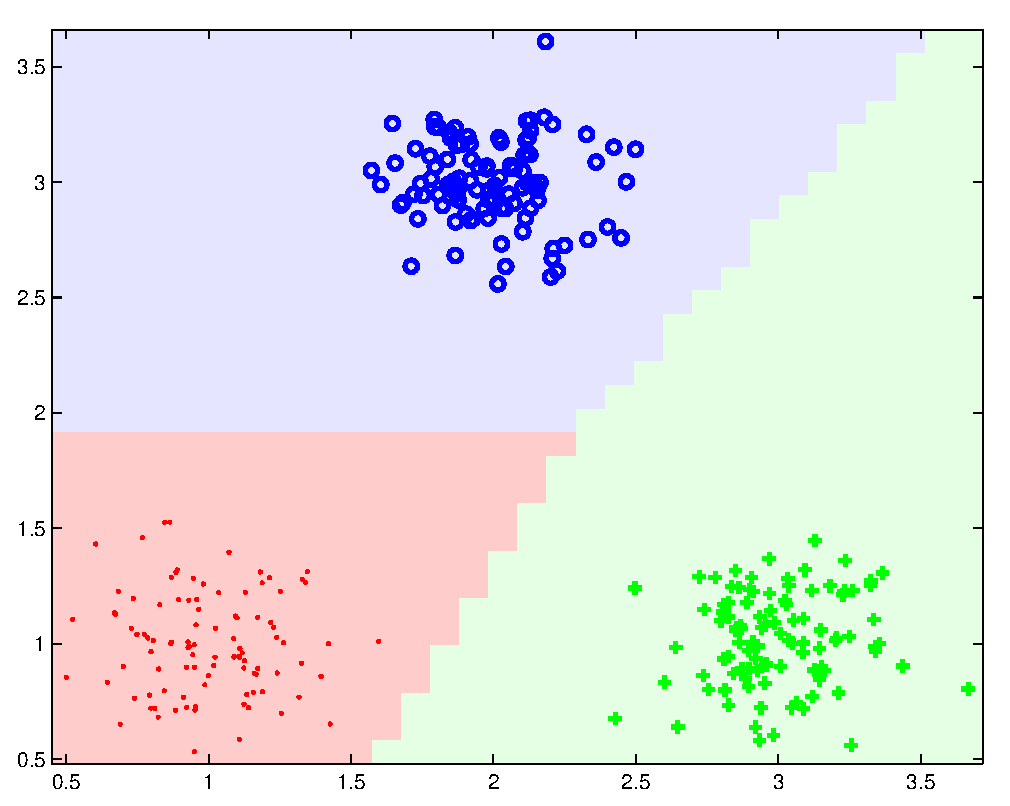
\includegraphics[scale=0.25]{{../eps/fig2_H2_eta0.001000}.eps}
\caption{ $H=2$}
\endminipage\hfill
\minipage{0.32\textwidth}
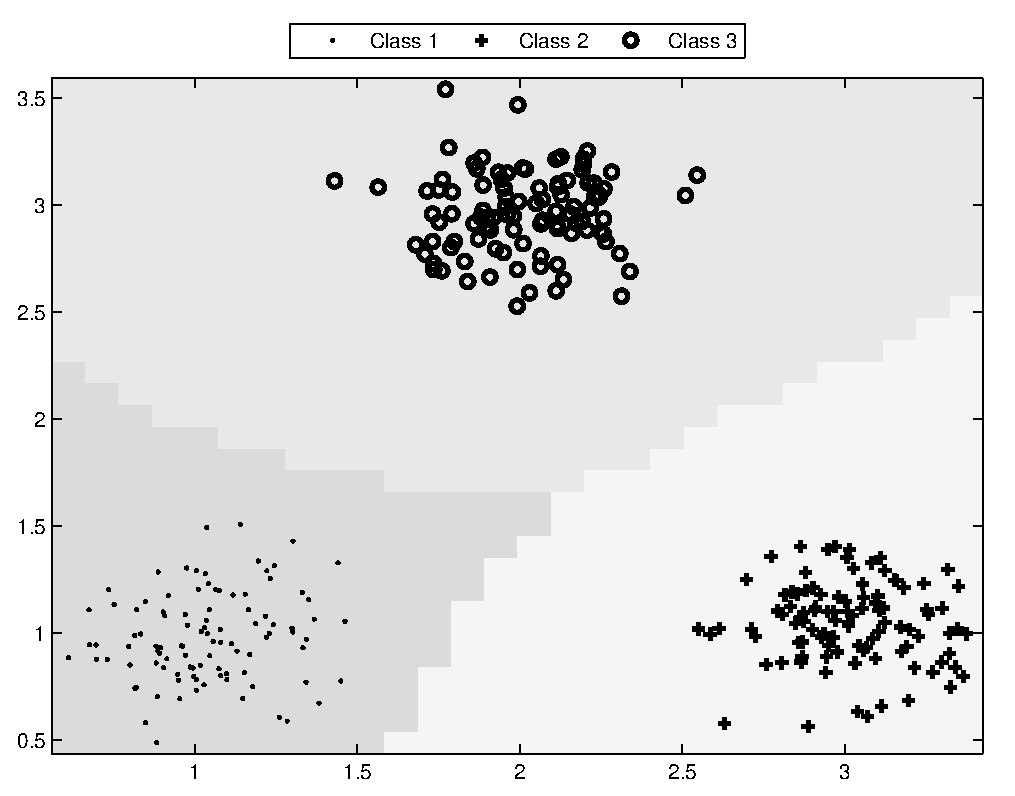
\includegraphics[scale=0.25]{{../eps/fig2_H4_eta0.001000}.eps}
\caption{ $H=4$}
\endminipage\hfill
\minipage{0.32\textwidth}
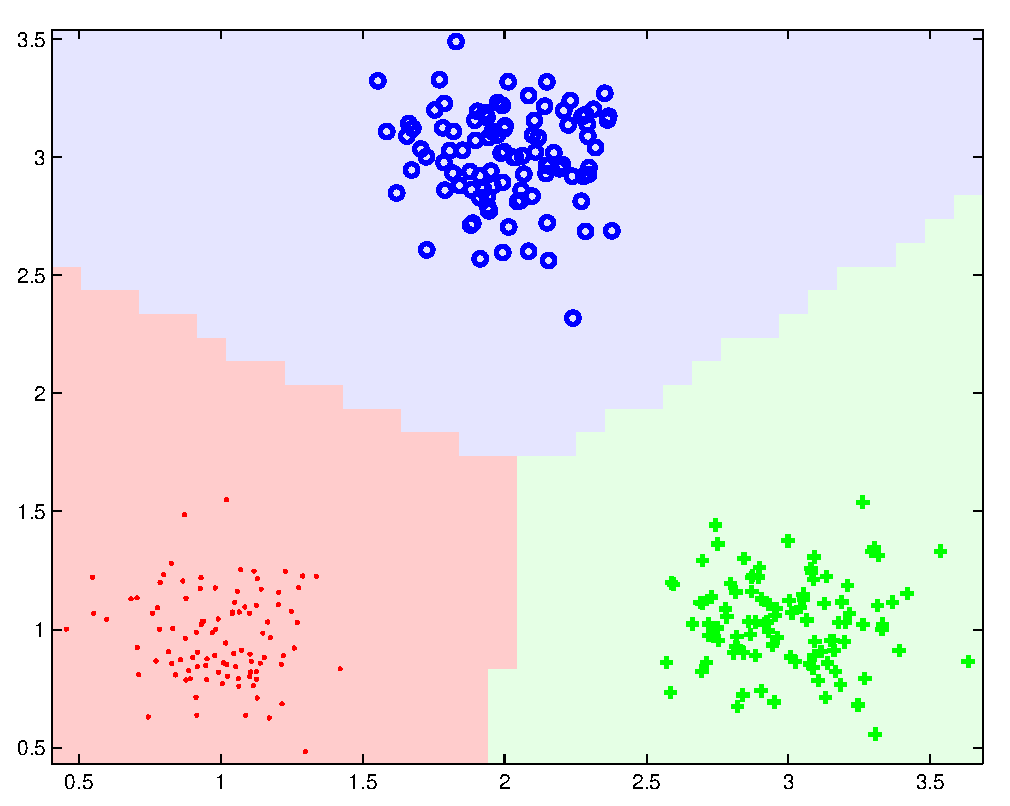
\includegraphics[scale=0.25]{{../eps/fig2_H64_eta0.001000}.eps}
\caption{ $H=64$}
\endminipage\hfill
\caption{Deicision boundary for $\eta=0.001$}
\label{fig:fig13}
\end{figure}

\begin{figure}[H]
\minipage{0.32\textwidth}
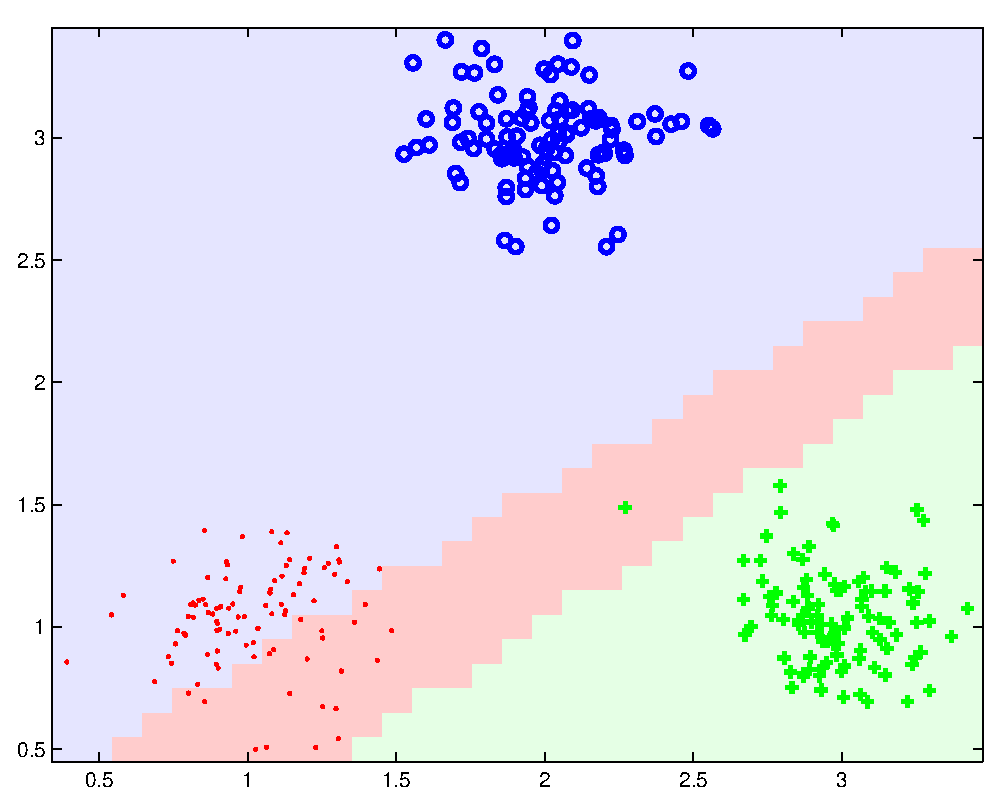
\includegraphics[scale=0.25]{{../eps/fig2_H2_eta0.000100}.eps}
\caption{ $H=2$}
\endminipage\hfill
\minipage{0.32\textwidth}
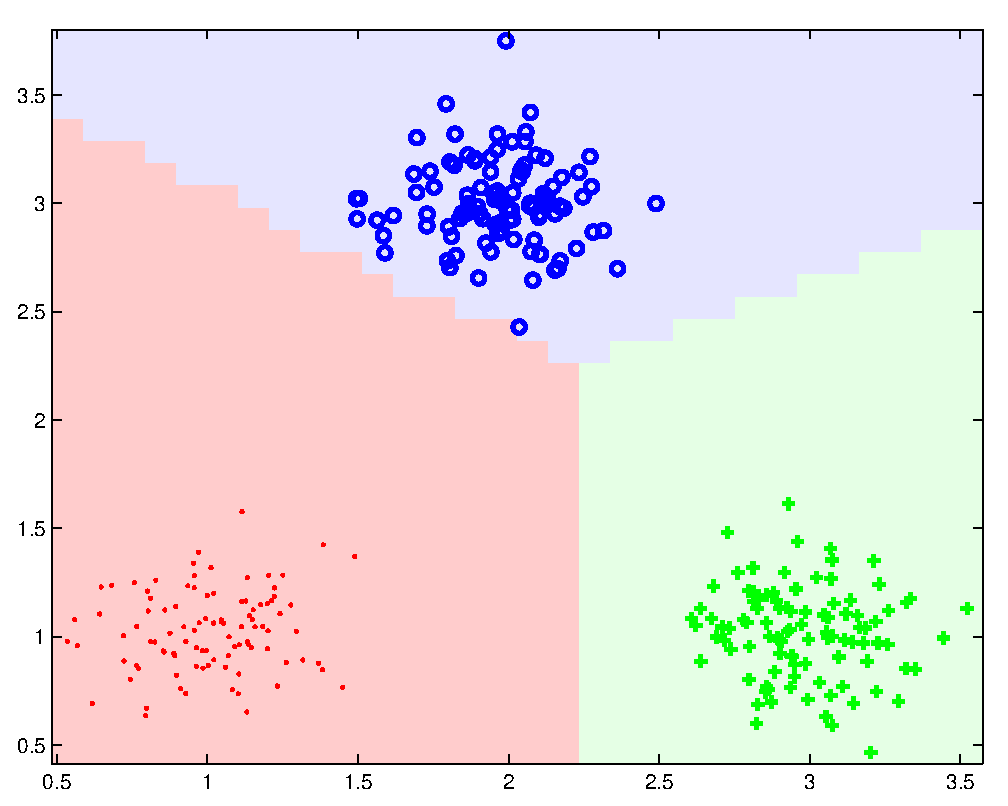
\includegraphics[scale=0.25]{{../eps/fig2_H4_eta0.000100}.eps}
\caption{ $H=4$}
\endminipage\hfill
\minipage{0.32\textwidth}
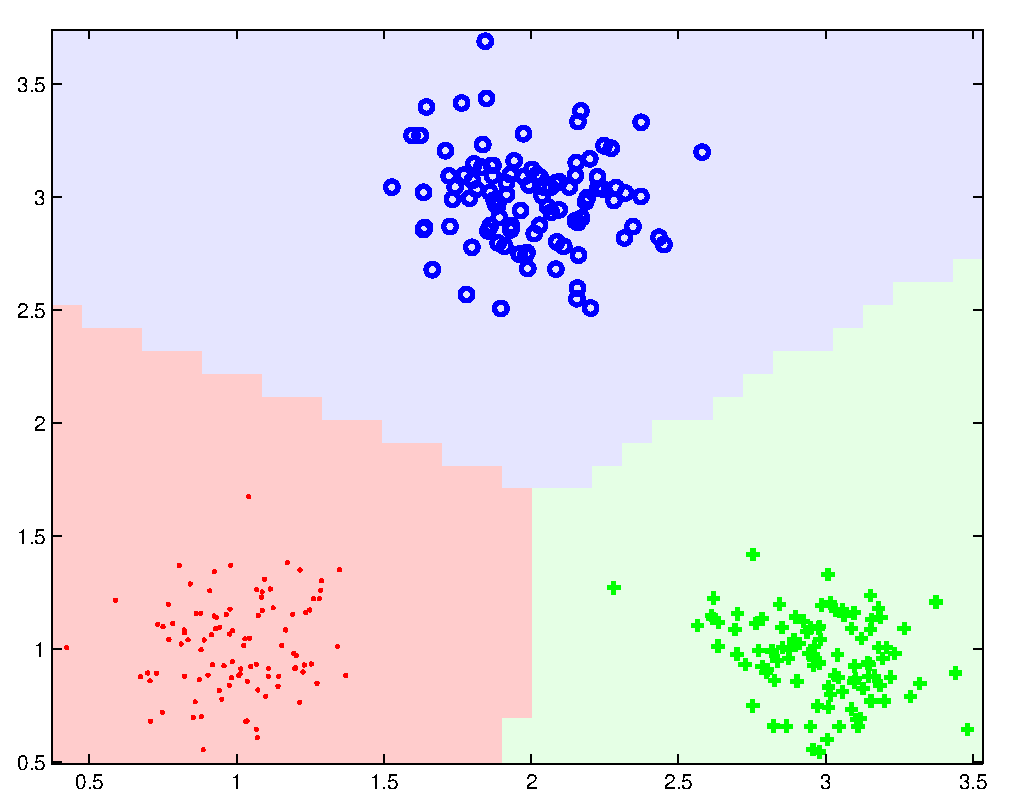
\includegraphics[scale=0.25]{{../eps/fig2_H64_eta0.000100}.eps}
\caption{ $H=64$}
\endminipage\hfill
\caption{Deicision boundary for $\eta=0.0001$}
\label{fig:fig14}
\end{figure}

\begin{figure}[H]
\minipage{0.32\textwidth}
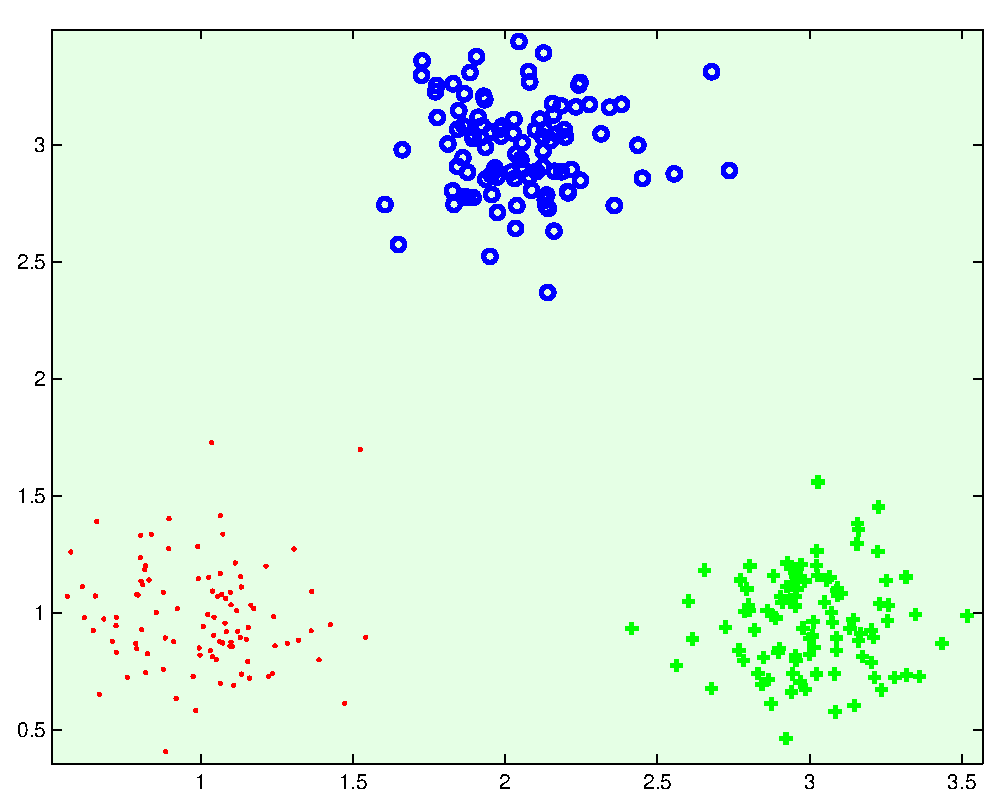
\includegraphics[scale=0.25]{{../eps/fig2_H2_eta0.000010}.eps}
\caption{ $H=2$}
\endminipage\hfill
\minipage{0.32\textwidth}
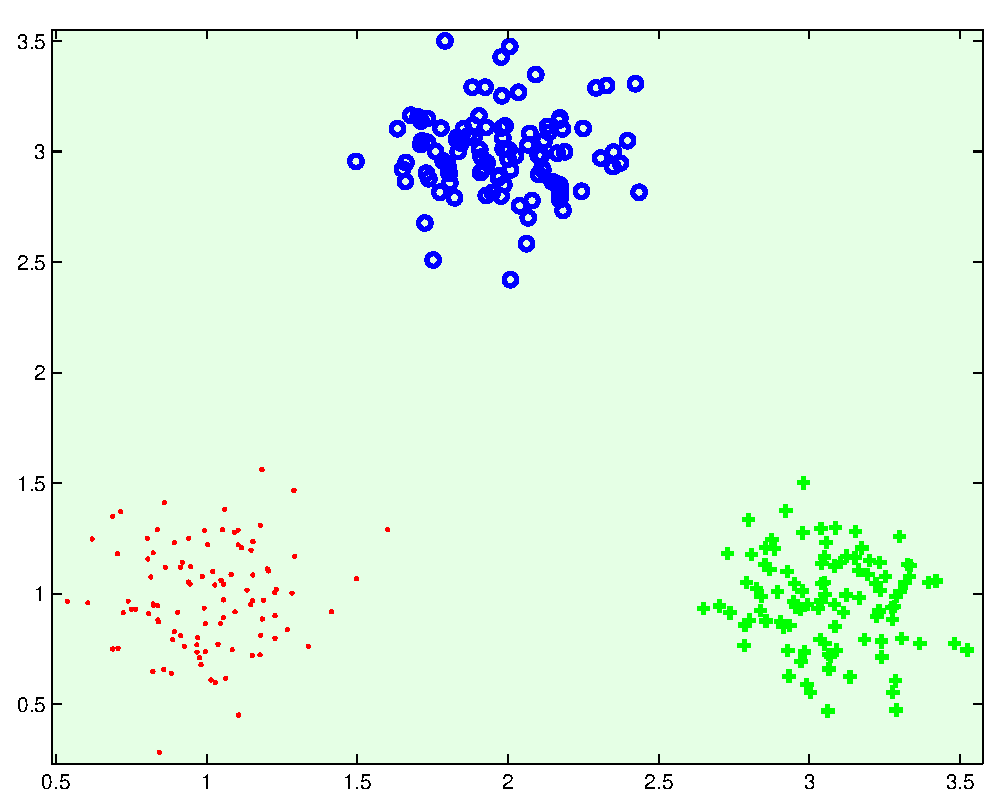
\includegraphics[scale=0.25]{{../eps/fig2_H4_eta0.000010}.eps}
\caption{ $H=4$}
\endminipage\hfill
\minipage{0.32\textwidth}
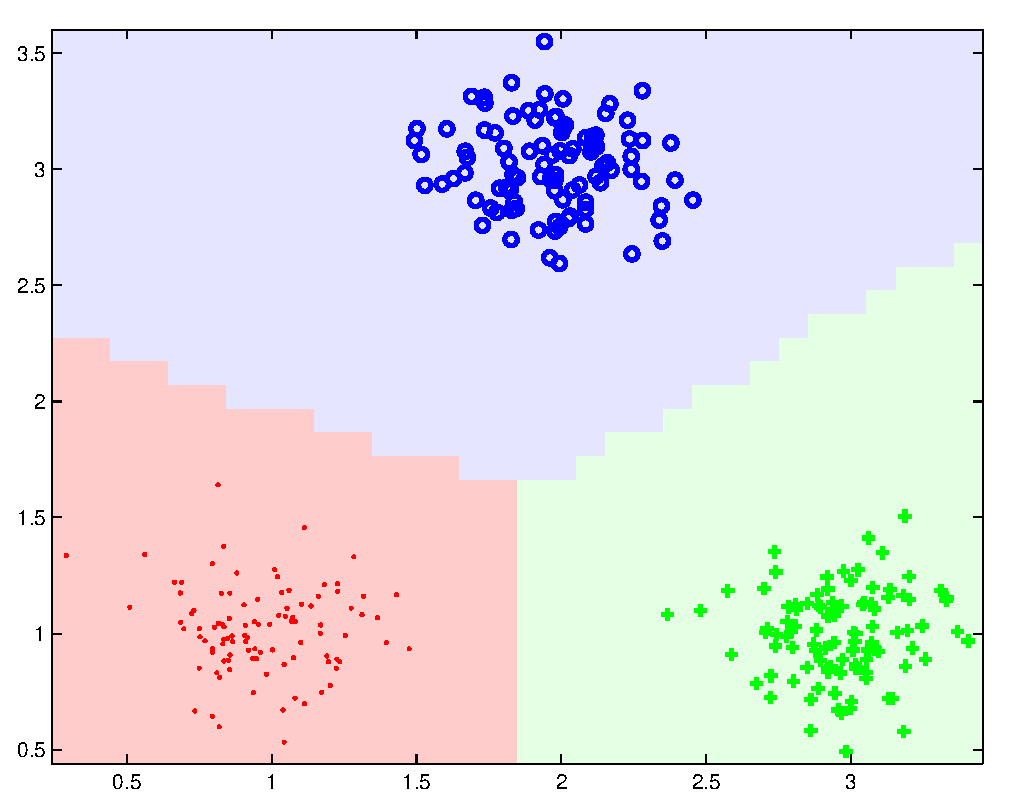
\includegraphics[scale=0.25]{{../eps/fig2_H64_eta0.000010}.eps}
\caption{ $H=64$}
\endminipage\hfill
\caption{Deicision boundary for $\eta=0.00001$}
\label{fig:fig15}
\end{figure}

\subsection{Discussion and Conclusions}
\subsubsection{Hidden Layer Nodes}
As we can see from Figure \ref{fig:fig1} and \ref{fig:fig2} increasing the number of hidden layer nodes increases the convergence rate for the neural network but in the end, all the networks become almost the same given sufficient iterations, although $H=64$ still dominates in all cases. However, in case of lower learning rate, networks with more number of hidden layer nodes are able to converge quickly in comparison to others as can be seen in Figures \ref{fig:fig3}, \ref{fig:fig4} and \ref{fig:fig5}. This is because the network will be able to represent more complex data with an increase in the number of hidden layer nodes which will represent various intermediate functions and representation of-of data (i.e. classification into classes) can be done quickly with more hidden layer nodes rather than taking more iterations with less number of hidden layer nodes. Also, this process will saturate and beyond a particular limit increasing the hidden layer nodes will not make any significant difference.

\subsubsection{Learning Rate}
As we can see from Figure \ref{fig:fig6}, \ref{fig:fig7}, \ref{fig:fig8}, \ref{fig:fig9}, \ref{fig:fig10} and \ref{fig:fig11}; increasing the learning rate leads to faster convergence. This is because the magnitude of the learning rate hasn't been too high to cause oscillations in the error space and hence increasing the learning rate within particular limits will only fasten the process of convergence of the network to a better solution.

\subsubsection{Training Iterations}
We are performing a stochastic gradient descent on the data which is based on finding the gradient with respect to a particular point and changing weights accordingly, this method will give better and better results as network is trained with more and more number of points, i.e. with increase in total iterations the error in the output of the network decreases as can be seen in all the Figures.

\subsubsection{Decision Boundary}
As we can see for appropriate learning rate all networks (i.e. varying them respect to the number of hidden layer nodes) give a very accurate description of decision boundary though they differ slightly in term of the structure and also the sum of squared errors. The reason for the latter is of the ability of networks with more complexity (more hidden layer nodes) give very strong probabilities in terms of output in case of the three classes whereas weaker networks give only mild probabilities everywhere, though the separating boundary can still remain same. We can also that though correct, weaker networks are ``unsure'' about their decision or are ``indecisive'' in cases. Also, here network with higher hidden layer nodes were able to get a nice decision boundary for even low learning rate as can be seen from Figures \ref{fig:fig12}, \ref{fig:fig13}, \ref{fig:fig14} and \ref{fig:fig15}. 

\section{Neural Network to predict the steering angle from the road image for a self-driving car}
\subsection{Network Structure}
If we consider the network to be composed of $n_1, n_2, ... n_k$ nodes in each layer with the corresponding vectors to be $\vec v_1,\vec v_2, ... \vec v_k$ and the weights for each layer be $ \vec w_1, \vec w_2, ... \vec w_{k-1}$, we can then say that $v_{ij}=\sigma(\vec w_{i-1,j}^T \vec v_{i-1}), i\in\{2,3,..k\}$. In other words: 
\begin{gather*}
\vec v_i=\begin{pmatrix}v_{i,1}\\v_{i,2}\\...\\v_{i,n_i}\end{pmatrix}_{n_i\times1},
\vec w_{i,j}=\begin{pmatrix}w_{i,1,j}\\w_{i,2,j}\\...\\w_{i,n_i,j}\end{pmatrix}_{n_i\times 1}\\
\vec w_{i}=\begin{pmatrix}\vec w_{i,1}^T\\\vec w_{i,2}^T\\...\\\vec w_{i,n_{i+1}}^T\end{pmatrix}_{n_{i+1}\times n_i}=\begin{pmatrix}w_{i,1,1}&w_{i,2,1}&...&w_{i,n_{i},1}\\w_{i,1,2}&w_{i,2,2}&...&w_{i,n_{i},2}\\\vdots&\vdots&\ddots&\vdots\\w_{i,1,n_{i+1}}&w_{i,2,n_{i+1}}&...&w_{i,n_i,n_{i+1}}\end{pmatrix}
\end{gather*}
where
\begin{align*}
\vec v_i&\text{ is Layer $i$}\\
v_{i,j}&\text{ is $j^\text{th}$ node in Layer $i$}\\
\vec w_i&\text{ is weight from Layer $i$ to $i+1$}\\
\vec w_{i,j}&\text{ is weight from Layer $i$ to $j^\text{th}$ node in Layer $i+1$}\\
w_{i,a,b}&\text{ is weight from $a^\text{th}$ node in Layer $i$ to $b^\text{th}$ node in Layer $i+1$}
\end{align*}
and thus
\begin{align*}
v_{i,j} &=\sigma(\vec w_{i-1,j}^T\vec v_{i-1})\\
&=  \sigma\left(
	(w_{i-1,1,j},w_{i-1,2,j},...,w_{i-1,n_{i-1},j})
	\begin{pmatrix}
		v_{i-1,1}\\v_{i-1,2}\\...\\v_{i-1,n_{i-1}}
	\end{pmatrix}
	\right)\\
&=\sigma\left(\sum_{l=1}^{n_{i-1}}w_{i-1,l,j}v_{i-1,l}\right)\\
\end{align*}
and
\begin{align*}
\vec v_i&=\begin{pmatrix}v_{i,1}\\v_{i,2}\\...\\v_{i,n_{i}}\end{pmatrix}
=\begin{pmatrix}\sigma(\vec w_{i-1,1}^T\vec v_{i-1})\\\sigma(\vec w_{i-1,2}^T\vec v_{i-1})\\...\\\sigma(\vec w_{i-1,n_i}^T\vec v_{i-1})\end{pmatrix}
=\vec \sigma\left(\begin{pmatrix}\vec w_{i-1,1}^T\vec v_{i-1}\\ \vec w_{i-1,2}^T\vec v_{i-1}\\ ...\\ \vec w_{i-1,n_i}^T\vec v_{i-1}\end{pmatrix}\right)\\
&=\vec \sigma (\vec w_{i-1}\vec v_{i-1})
\end{align*}

\begin{figure}[H]
\centering
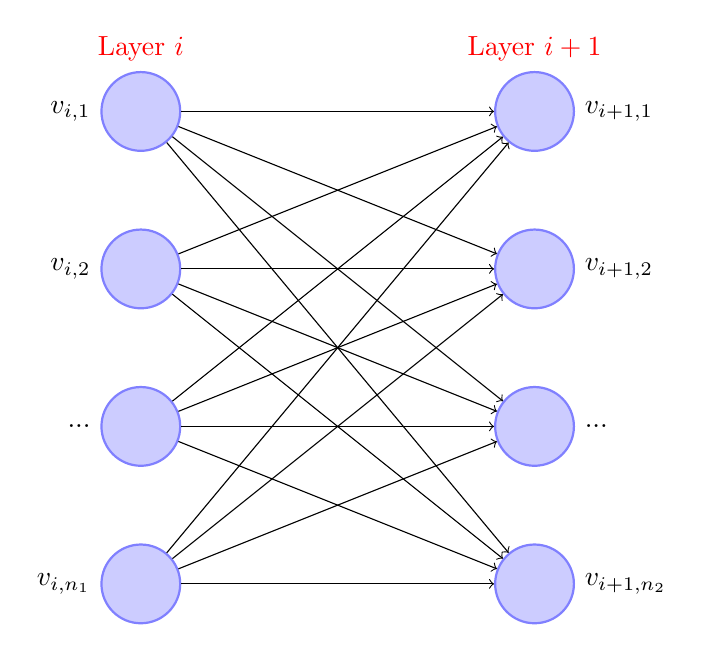
\begin{tikzpicture}
[auto, nd/.style = {circle,minimum size=1cm,draw=blue!50,fill=blue!20,thick}]

\foreach \n/\name in {1/1,2/2,3/x,4/{$n_1$}}
		\node[nd] (I\n) at (0,-2*\n) [label=left:{ \ifthenelse{\equal{\name}{x}}{{...}}{$v_{i,\text{\name}}$} }] {};
		
\foreach \n/\name in {1/1,2/2,3/x,4/{$n_2$}}
		\node[nd] (J\n) at (5,-2*\n) [label=right:{ \ifthenelse{\equal{\name}{x}}{{...}}{$v_{i+1,\text{\name}}$} }] {};		
		
\foreach \i/\o in {1/1,2/2,3/x,4/{$n_1$}}{
	\foreach \j/\k in {1/1,2/2,3/x,4/{$n_2$}}{
		\draw [->] (I\i) -- (J\j);
	}
}

\node[red,above] at (I1.north) {Layer $i$};
\node[red,above] at (J1.north) {Layer $i+1$};

\end{tikzpicture}
\caption{Portion of a neural network from layer $i$ to layer $i+1$. The weight used here will be $\vec w_i$.}
\end{figure}
\subsection{Gradient Descent}
The error term for a minibatch of size $n$ (i.e. from $j$ to $j+n-1$) would be:
$$E = \sum_{i=j}^{j+n-1}\frac 12 || o^i- v_{k}^i||^2$$
where superscript $i$ denotes the $i$-th point.
For a particular point the error would be:
$$\frac 12 || o- v_{k}||^2=\frac 12\sum_{l=1}^{n_k}(o_{l}-v_{k,l})^2$$
The gradient wrt weights $w_{k-1,a_{k-1},a_{k}}$ can be obtained using chain rule:\\
$$\frac{\partial E}{\partial w_{k-1,a_{k-1},a_{k}}}=\underbrace{(v_{k,a_k}-o_{a_k})v_{k,a_k}(1-v_{k,a_k})}_{\delta_{k,a_k}}v_{k-1,a_{k-1}}$$
Similarly for any previous layer we can obtain:\\
$$\frac{\partial E}{\partial w_{i,a_i,a_{i+1}}}=\underbrace{\sum_{a_{i+2}=1}^{n_{i+2}} \delta_{i+2,a_{i+2}}w_{i+1,a_{i+1},a_{i+2}}}_{\delta_{i+1,a_{i+1}}}v_{i,a_i}$$
and wrt a particular point\\
$$\Delta w_{i,a_i,a_{i+1}}=\eta \delta_{i+1,a_{i+1}}v_{i,a_i}$$
For minibatch gradient descent we would add up these $\Delta w_{i,a_i,a_{i+1}}$'s. Also note that we also have some biases that would not propagate the gradient backwards so in case of calculation of $\delta_{i,a_i}$ we would neglect the term coming from $v_{a_{i+1}}=1$ i.e. the bias term of the $i+1$-th layer.

Now we find a relation between $\delta_{i,j}$'s. We define $\vec \delta_i$ as follows:
$$\vec \delta_i=\begin{pmatrix}\delta_{i,1}\\\delta_{i,2}\\...\\\delta_{i,n_i}\end{pmatrix}_{n_i\times 1}$$
And we define $\delta_{i,j}$ as follows:
$$\delta_{i,j}=\begin{cases}(v_{k,j}-o_j)v_{k,j}(1-v_{k,j})&i=k\\\displaystyle\sum_{x=1}^{n_{i+1}}\delta_{i+1,x}w_{i,j,x}&\text{otherwise}\end{cases}$$
We can observe that:
\begin{gather*}\Delta\vec w_{i}=\eta \vec \delta_{i+1}\vec v_{i}^T\\
\vec\delta_i=\vec w_i^T\vec \delta_{i+1}
\end{gather*}
\subsection{Minibatch gradient Descent}
We define few more quantities (here superscript $i$ denotes $i$-th point, $n$ denotes total points in a minibatch):
\begin{gather*}
\vec V_i = \begin{pmatrix}\vec v_i^1&\vec v_i^2&...&\vec v_i^n\end{pmatrix}\\
\vec \xi_i =\begin{pmatrix}\vec \delta_i^1&\vec \delta_i^2&...&\vec \delta_i^n\end{pmatrix}
\end{gather*}
We note that:
\begin{gather*}
\vec V_i = \vec \sigma (\vec w_{i-1}^T \vec V_{i-1})\\
\vec \xi_i = \vec w_i^T\vec \xi_{i+1}\\
\Delta \vec w_i = \eta\vec \xi_{i+1} \vec V_{i}^T=\eta \sum_{j=1}^n\vec \delta_{i+1}^j\vec v_i^{j,T}
\end{gather*}
\end{document}